\documentclass[12pt]{article}
\usepackage{footnote}
\usepackage{chngpage}
\usepackage{graphicx}
\makesavenoteenv{tabular}
\title{Analysis of the feasability of brute-forcing DES on consumer-grade hardware }

\author{Doug Johnson\\
CS 5460 Computer Security\\
Utah State University, Logan UT, USA\\
dougvj@gmail.com\\
}

\date{December 3, 2012}

\begin{document}
\maketitle

\begin{abstract}
The rapid development of computing ability on consumer grade hardware, especially in the area of using Graphics Processing Units (GPUs) for general purpose computing using OpenCL, has rendered today's enthusiast PC at or near the level of the super computers of the late 90s. In this report, I document my implementation of DES in C and OpenCL for the purposes of benchmarking and determining the feasability of brute-force key search attack on DES encryption using my own PC hardware. 
\end{abstract}

\section{Introduction}
OpenCL is a recent programming language standard produced as a result of the sudden popularity of using Graphics Processing Units for general purpose computing, not only in academic and scientific computing, but also amoung consumers where it can be used to accelerate video game physics, photo and audio manipulation, and encryption and decryption.

OpenCL's use in security applications like accelerating encryption leads to valid concerns. Exhaustive key search becomes more feasible for smaller key-spaces, most notably DES. DES has been demonstrably insecure ever since the Electronic Frontier Foundation designed and build special purpose hardware that was able to exhaust the keyspace and found the key in a mere couple of days. This hardware, however, was expensive and chartered for this particular purpose. A combination of cheaper and faster consumer-grade hardware as well as optimizations in software has brought us closer to the point where an average consumer will be perform a brute force DES search, possibly within the next decade, while today it is certainly possible to break DES without specialty hardware for under \$10000.  

\section{Procedure}
The first step was to create a fast and eifficient DES implementation in traditional software. I chose C for its and simplicity over more obfuscating objected oriented or managed languages. The initial implementation took about 4 hours, and another 5 hours of testing was required in order for the implementation to be correct. The testing was done with custom unit testing and reference encryption examples. Once this was complete, code for multithreaded brute-forcing as well as becnhmarking was created.

Once the implementation in C was correct and complete, I proceeded to port it to OpenCL. OpenCL is C-like enough that for most of the code, simple replacement of keywords and datatypes was needed. OpenCL is unique in that for most devices it is more eifficient to use vector data-types than it is to use scalars. For that reason, the OpenCL algorithm uses a 4 component vector on which all operations are carried out and 4 encryptions/decryptions can be carried out by the same hardware core simultaneously. Some adjustments had to be made, most notably in the sboxes step, for the vector types. This step took about an hour.

At his point, I added to the C code's library interface to support OpenCL, and added test cases which compare the OpenCL output with that of the C code. About 2 hours were spent debugging the OpenCL code, mostely on the C side, including complications with OpenCL thread scheduling and memory transfers.

At this point, additional debugging was needed for testing the program between different platforms, and careful recording of benchmark results on various devices was carried out.


\section{Results}
The benchmarking code has been executed on multiple devices. For each device, the keys per second which can be checked is benchmarked. Below is a table summarizing the results:
\begin{savenotes}
\begin{table}[h]
\tiny
\begin{adjustwidth}{-5in}{-5in}
\centering
\begin{tabular}{|l|c|c|c|c|r|r|r|}
\hline
%%%%%%%%%%%%%%%%%%%%%%%%%%%%%%%%%%%%%%%%%%%%%%%%%%%%%%%%%%%%%%%%%%%%%%
%%                                                                  %%
%%  This is a LaTeX2e table fragment exported from Gnumeric.        %%
%%                                                                  %%
%%%%%%%%%%%%%%%%%%%%%%%%%%%%%%%%%%%%%%%%%%%%%%%%%%%%%%%%%%%%%%%%%%%%%%
Name	&Year Released	&Clockspeed (MHz)	&Codename	&Architecture	&Num Keys	&Time (s)	&Keys/Sec\\ \hline
Athlon XP 1500+	&2001 Q4	&1x1333	&Palomino	&ia32	&102,400,000	&3490.570	&29,336\\
Intel Core 2 Duo T7200	&2006 Q3	&2x2000	&Memrom	&AMD64	&102,400,000	&1209.620	&84,655\\
Nvidia 8800GTS	&2006 Q4	&	&G80	&	&102,400,000	&24.594	&4,163,556\\
Intel Core 2 Quad Q6600	&2007 Q1	&4x2400	&Kentsfield	&AMD64	&102,400,000	&468.921	&218,374\\
Intel Xeon X3350	&2008 Q1	&4x2666	&Yorkfield	&AMD64	&102,400,000	&130.861	&782,507\\
Atom N270	&2008 Q3	&1x1600	&Diamondville	&ia32	&102,400,000	&3400.634	&30,112\\
AMD Radeon HD 6950	&2010 Q4	&	&Cayman	&	&102,400,000	&6.569	&15,587,973\\
Intel Core i7 2620M	&2011 Q1	&2x2700	&Sandy Bridge	&AMD64	&102,400,000	&187.283	&546,767\\
Qualcomm Scorpion	&2011 Q2	&2x1200	&	&ARM v7	&102,400,000	&31963.89	&32,365\\
BCM2708 (Raspberry PI)	&2012 Q1	&1x700	&	&ARM v6	&12,800,000	&1383.590	&9,251\\
Intel Core i7 3770K 3.5GHz	&2012 Q2	&4x3500	&Ivy Bridge	&AMD64	&102,400,000	&60.213	&1,700,618\\
AMD FX 8350	&2012 Q3	&8x4400	&Piledriver	&AMD64	&102,400,000	&50.449	&2,029,762\\
\hline

\end{tabular}
%\caption{DES Decryption performance on various devices}
\label{tab:myfirsttable}
\end{adjustwidth}
\end{table}
\end{savenotes}

On as many computational devices as possible, the author executed the benchmarking code to determine the speed of various consumer devices, including even mobile phones. Access to OpenCL Compute devices is very difficult to obtain, and therefore only two, both of which the author owns, have been represented. Plots of the data are given in the appendix.

The first and most interesting aspect of all these benchmarks is that a single 
device more than doubles the power of all the other devices combined. This is
a consumer graphics card, an AMD Radeon HD 6950. This card, interestingly enough,
is no longer being manufactured as it has been superceded by the new HD 7000 series
which is about 70\% faster according to most benchmarks. This clearly shows the
massive increase in compute power that an enthusiast GPU provides over standard
CPUs. The other GPU tested, an nVidia geForce 8800GTS, has a release date of 6 years
ago and still doubles the performance of the fastest CPU tested.

Unfortunately with all of the devices on the chart running simultaneously and fulltime,
it would take 90.61 years to perform and exhaustive key-space search with an average time
of 45.31 years to find the key. With the HD 6950 alone, these numbers would be 146.58
and 74.29 years respectively. This clearly is not practical for DES cracking, 
however, there are some factors that can make it more practical.

This first involves software optimizations. In 1997 Dr. Eli Biham in a conference
on encryption performance presented a paper on a new fast DES implementation
\footnote{http://www.cs.technion.ac.il/users/wwwb/cgi-bin/tr-info.cgi/1997/CS/CS0891}
. The technique involves what has been coined as 'bitslicing', 64 64-bit blocks
are encrypted-decrypted simultaneously by treating a single 64-bit block in hardware
as representing the same bit of all 64-bit blocks, that is, block one has 64-bits,
all of which represent bit 1 of their respective block. This allows DES to be
implemented as a series of gate operations on each bit. This is quite eifficient
in software. Permutations can be simple pointer references and SBox operations
are reduced to gate operations tuned to each bit. This implementation, according to Biham,
averages about double the speed of standard implementation speeds, avoiding expensive
permutation and sbox operations.

Biham estimates that the fastest supercomputer of the time, Sandia's ASIC Red,
could do and exhaustive key search in about 6 months. Biham further claims that
a 133 MHz RISC processor, representing an average CPU on the internet at the time,
could encrypty/decrypt $2^{18}$ keys per second. This author is very skeptical of
such estimates, and believes that with this code running on a 133 MHz processor
the performance would be on the order of 2000 keys/sec. With optimizations it is 
highly unlikely that the processor would ever approach the $2^{18}$ estimate, however
impromtu tests with a modified DES algorithm without permutations shows a speed 
increase of over an order of magnitude, therefore it is possible that Biham's 
method of implementation in some circumstances can show similar gains.

 Brandon et al\footnote{http://www.researchgate.net/publication/220922662\_AES\_and\_DES\_Encryption\_with\_GPU/file/d912f5062ed3d4c86b.pdf} implemented DES on a GPU when it was first gaining traction in 
2008. Their implementation shows performance at the same order of magnitude as mine. Agosta et al
\footnote{http://csis.bits-pilani.ac.in/faculty/murali/netsec-11/seminar/refs/rahul7.pdf} provided an implementation on GPUs that approached 300 million keys per second on a single device.

Perhaps more notable than raw numbers is the vast speed gains we can see as a function of time.
Hardware from 1997 using my code would likely provide a mere 10000 or so keys per second.
The Raspberry PI was the worst performer in the table; The Raspberry PI foundation estimates that the
PIs CPU is equivalent to a 300 MHz Pentium II in performance. This CPU was mainstream in about 1997.
Compute power has clearly seen massive gains, and it is reasonable to predict that, using my code,
in 2027 high end devices in software will be able to produce performance on the order of 5 billion
keys per second on an enthusiast machine. This will 
be enough compute power to find a key in a matter 
of a couple months. 

Although an average PC may not be able to practically crack DES, it is clear that anyone with
moderate resources can build a compute cluster out of GPUs, or even an ad hoc cluster using 
existing computer networks, can break DES in a reasonable amount of time. A high end PC with 4 consumer 
graphics cards using my code will be able to check around 70 million keys per second. With optimizations
this estimate can be safely doubled. This will be enough to crack DES in 16 years. With 16 PCs, this will be
reduced to a year. Building this can be done for about \$30000. At the moment it is
more economical to use FPGA hardware to build a custom cracking machine, as demonstrated
with project COPACOBANA.\footnote{http://www.copacobana.org/paper/TC\_COPACOBANA.pdf}

\section{Conclusion}

Although the scope of this project excludes advanced optimizations that may be specifically used
for DES brute-forcing, it demonstrates the incredible gains that computing has made in the past
decade in a half and the emerging use of parallelization in encryption applications. Although for
the time being it is more practical and economical to develop custom hardware or FPGA systems to
crack DES, pre-existing general purpose enthusiast PC hardware will be able to economically
crack DES within the next decade.




%\begin{adjustwidth}{-5in}{-5in}
%\centering
%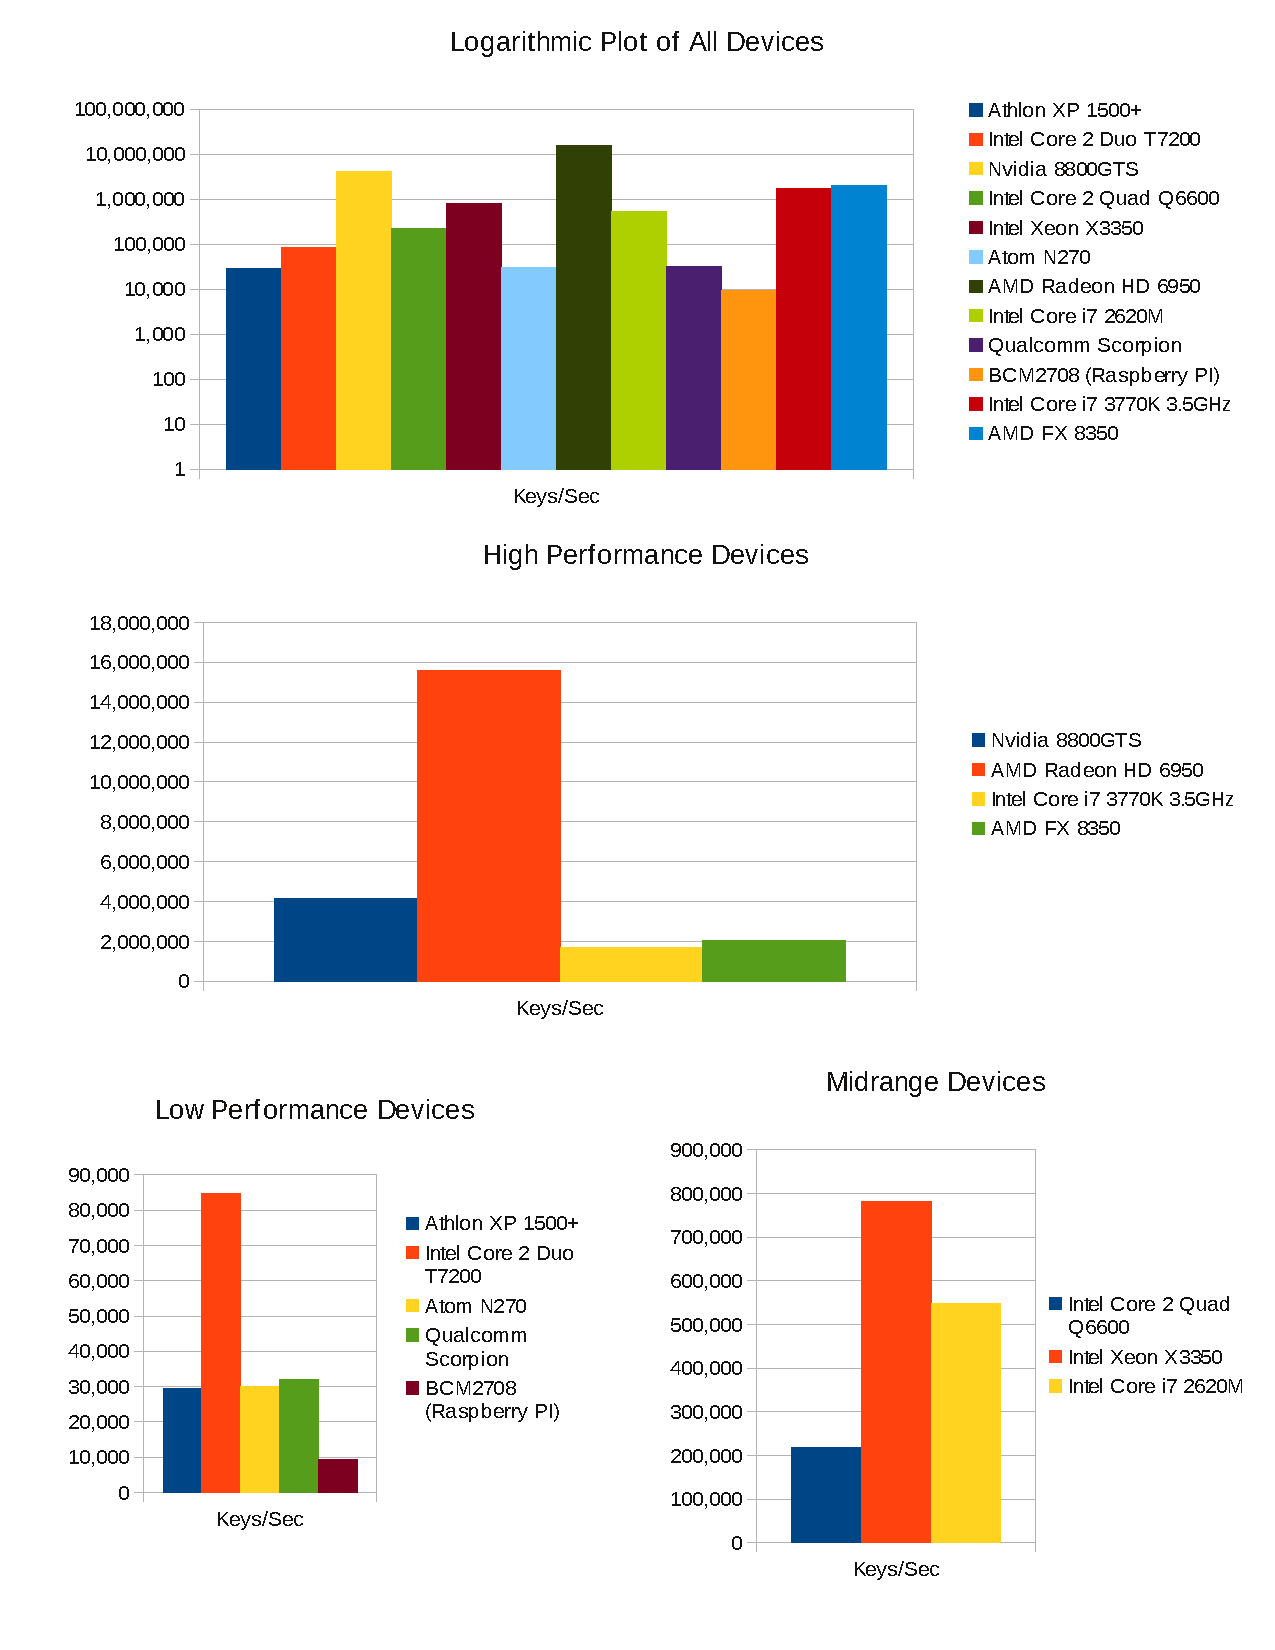
\includegraphics{figures.pdf}
%\end{adjustwidth}

\end{document}

